\documentclass[8pt, twocolumn]{article}
\usepackage[margin=1in]{geometry}
\usepackage{lmodern}% http://ctan.org/pkg/lm
\usepackage{authblk} % adds affiliations

\usepackage[utf8x]{inputenc}
\usepackage{nameref}
\usepackage[switch]{lineno}
\usepackage{amsmath}
\usepackage{booktabs}
\usepackage[numbers,super]{natbib}
\usepackage{changepage}

% adjust caption style
\usepackage[aboveskip=1pt,labelfont=bf,
            labelsep=period,singlelinecheck=off]{caption}

% remove brackets from references
\makeatletter
\renewcommand{\@biblabel}[1]{\quad#1.}
\makeatother

\usepackage[colorinlistoftodos]{todonotes}

% headrule, footrule and page numbers
\usepackage{lastpage,fancyhdr,graphicx}
\usepackage{epstopdf}
\pagestyle{myheadings}
\pagestyle{fancy}
\fancyhf{}
\rfoot{\thepage/\pageref{LastPage}}
\renewcommand{\footrule}{\hrule height 2pt \vspace{2mm}}

% use \textcolor{color}{text} for colored text (e.g. highlight to-do areas)
\usepackage{color}

\definecolor{Gray}{gray}{.25}

\usepackage{graphicx}

% use if you want to put caption to the side of the figure
\usepackage{sidecap}

\usepackage{xcolor}
\usepackage[colorlinks = true,
            linkcolor = blue,
            urlcolor  = blue,
            citecolor = blue,
            anchorcolor = blue]{hyperref}

% ####################################################
% ####################################################
\usepackage[colorinlistoftodos]{todonotes}
% ####################################################
% ####################################################

% use for have text wrap around figures
\usepackage{wrapfig}
\usepackage[pscoord]{eso-pic}
\usepackage[fulladjust]{marginnote}
\reversemarginpar{}

\usepackage{gensymb}
\usepackage{siunitx}

% make a box for author summary
\usepackage[framemethod=TikZ]{mdframed}
%% define the style
\newcommand{\mybox}[2]{%
         \begin{center}%
            \begin{tikzpicture}%
                \node[rectangle, draw=#1, top color=#1!10, bottom color=#1!10,
                      rounded corners=5pt, inner xsep=5pt, inner ysep=6pt,
                      outer ysep=10pt]{
                        \begin{minipage}{1\textwidth}#2\end{minipage}};%
            \end{tikzpicture}%
         \end{center}%
}

% new commands
% q value
\newcommand{\qval}[1]{$q<10^{-#1}$}

% species names
\newcommand{\cel}{\emph{C.~elegans}}
\newcommand{\dicty}{\emph{D.~discoideum}}
\newcommand{\ecol}{\emph{E.~coli}}
\newcommand{\gf}{gain-of-function allele}
\newcommand{\lf}{loss-of-function allele}
\newcommand{\strong}{strong loss-of-function allele}
\newcommand{\weak}{weak loss-of-function allele}

% gene names
% \newcommand{\gene}[1]{\emph{#1}} # for MS word typesetting
\newcommand{\gene}[1]{\mbox{\emph{#1}}}
\newcommand{\genotype}[1]{\mbox{\emph{#1}}}
\newcommand{\protein}[1]{\mbox{\uppercase{#1}}}
\newcommand{\ras}{\gene{let-60} (\emph{ras})}
\newcommand{\rasp}{\protein{let-60}}
\newcommand{\dpy}{\gene{mdt-12}}
\newcommand{\letgfn}{3,021}
\newcommand{\letlfn}{857}
\newcommand{\letgf}{\gene{let-60(gf)}}
\newcommand{\letlf}{\gene{let-60(lf)}}
\newcommand{\strongn}{2,863}
\newcommand{\weakn}{481}
\newcommand{\transn}{2,214}


% more space between rows
\newcommand{\ra}[1]{\renewcommand{\arraystretch}{#1}}

\title{A study of allelic series using transcriptomic phenotypes}

\author[1]{David Angeles-Albores}
\author[1,*]{Paul W. Sternberg}
\affil[1]{Division of Biology and Biological Engineering, Caltech,
Pasadena, CA, 91125, USA}
\affil[*]{Corresponding author. Contact: pws@caltech.edu}
\renewcommand\Affilfont{\itshape\small{}}

% document begins here
\begin{document}
% title

\twocolumn[
  \begin{@twocolumnfalse}
    \maketitle
    % \section*{Abstract}
    \textbf{Although transcriptomes have recently been used to perform epistasis
    analyses, they are not yet used to study intragenic function/structure
    relationships. We developed a theoretical framework to study allelic
    series using transcriptomic phenotypes. As a proof-of-concept, we apply our
    methods to an allelic series of \dpy{}, a highly pleiotropic Mediator subunit
    gene in \emph{Caenorhabditis~elegans}. Our methods identify functional units
    within \dpy{} that modulate Mediator activity upon various genetic modules.
    }
    \vspace{3mm}

  \end{@twocolumnfalse}
]


\linenumbers{}
\section*{Introduction}
An `allelic series' refers to a set of alleles with different phenotypes and can
be used to understand the functions encoded within a single gene regardless of
the molecular nature of the alleles used. Briefly, in an allelic series a set of
alleles are used to generate a set of homozygotes. These genotypes are used to
explore the number and severity of phenotypes encoded by the alleles in
question. Using the homozygote genotypes, the alleles can be ordered by severity
of effect relative to the wild type allele for each measured phenotype. Then,
\emph{inter se} \emph{trans}-heterozygotes are used to establish dominance
(complementation) hierarchies within the allele set for each phenotype in
question. Together, the severity and dominance hierarchies are used to infer
intragenic functional units. Allelic series have been used to study the dose
response curve of a phenotype for a particular gene and to infer null phenotypes
from hypomorphs. In \emph{Caenorhabditis~elegans}, the \gene{let-23},
\gene{lin-3} and \gene{lin-12} allelic series stand out as
examples~\cite{Aroian1991,Ferguson1985a,Greenwald1983}.

Biology has moved from expression measurements of single genes towards
genome-wide measurements. Expression profiling via
RNA-sequencing~\cite{Mortazavi2008} (RNA-seq) enables simultaneous measurement
of transcript levels for all genes in a genome. These measurements can be made
on a whole-organism scale or on single cells~\cite{Tang2009,Schwarz2012}.
Transcriptomes have been successfully used to identify new cell or organismal
states~\cite{Angeles-Albores2017,Villani2017} and  both methods can be used for
epistasis analysis~\cite{Dixit2016,AngelesAlboresHIF}.

As a proof of principle, we selected three alleles~\cite{Zhang2000,Moghal2003}
of a Mediator complex subunit in \cel{}, \dpy{}. Mediator is a macromolecular
complex that contains approximately 25 subunits~\cite{Jeronimo2017} and which
globally regulates RNA polymerase II (Pol II)~\cite{Allen2015,Takagi2006}. The
Mediator complex consists of four biochemical modules: the Head, Middle and Tail
modules and a CDK-8-associated Kinase Module (CKM). The CKM can associate
reversibly with the other modules, and it appears to inhibit
transcription~\cite{Knuesel2009,Elmlund2006}. In \cel{}, the CKM consists of
\protein{cdk-8}, \protein{mdt-13}, \protein{cic-1} and
\protein{DPY-22}~\cite{Grants2015}. \dpy{} acts in the formation of the male
tail~\cite{Zhang2000}, where it interacts with the Wnt pathway, and in vulval
formation~\cite{Moghal2003a}, where it inhibits the Ras pathway. Studies in the
male tail were carried out using allele \gene{dpy-22(bx93)}, which generates a
truncated \protein{dpy-22} protein as a result of a premature stop codon,
Q2549Amber~\cite{Zhang2000}. However, animals homozyguous for this allele
grossly appear phenotypically wild-type. In contrast, animals homozyguous for
the \gene{dpy-22(sy622)} allele, which encodes a premature stop codon,
Q1698Amber~\cite{Moghal2003},
% (see Fig.~\ref{fig:dpy22})
are dumpy (Dpy), have
egg-laying defects (Egl) and a multivulva (Muv) phenotype. Due to its
pleiotropic effects, a conclusive allelic series analysis has not previously
been performed.

% \begin{figure}
%   \centering{}
%   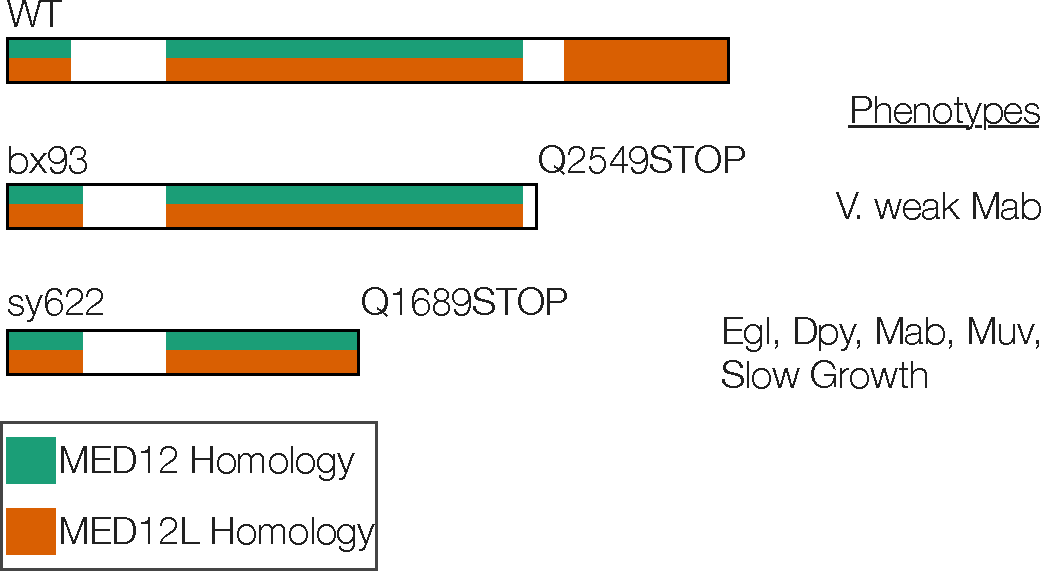
\includegraphics[width=0.3\textwidth]{../../figs/gene_model_dpy22.pdf}
%   \caption{
%     The \dpy{} allelic series, consisting of two amino acid truncations. Diagram
%     of the \protein{mdt-12} wild-type protein and the protein product of
%     \emph{bx93} and \emph{sy622} alleles.
%     % Conservation between \protein{mdt-12} and a human ortholog is shown in color.
%     }
% \label{fig:dpy22}
% \end{figure}

Expression profiles have the potential to facilitate dissection of molecular
structures within genes, but the high dimensionality of these phenotypes make
analysis challenging. We developed a framework to analyze allelic series using
transcriptomic phenotypes and applied our methods to a series involving the
MDT12 ortholog in \cel{}, \dpy{}. Our analysis revealed a number of functional
units that act to modulate Mediator activity at thousands of genetic loci.


\section*{Results}
% \subsection*{A conceptual framework for analyzing allelic series}
Allelic series offer a way to study the functional units within a gene without
requiring prior knowledge about the molecular structure of the mutations
involved. In an allelic series, a set of alleles are selected. Then, homozygotes
of each allele are generated (if possible), the phenotypes of each homozygote
are enumerated and their severity scored to order the alleles by loss (or gain)
of function relative to the wild-type allele. Finally, alleles are placed in
\emph{trans} to each other to check whether one allele is dominant or
semidominant over the other for each phenotype, resulting in an ordered
dominance hierarchy. This dominance hierarchy can be used to identify functional
units and their sequence requirements within a gene. We adapted this
methodology, which has been successfully used for scalar phenotypes, to be used
in conjunction with expression profiles (see Fig.~\ref{fig:flowchart}).

\begin{figure*}
  \centering{}
  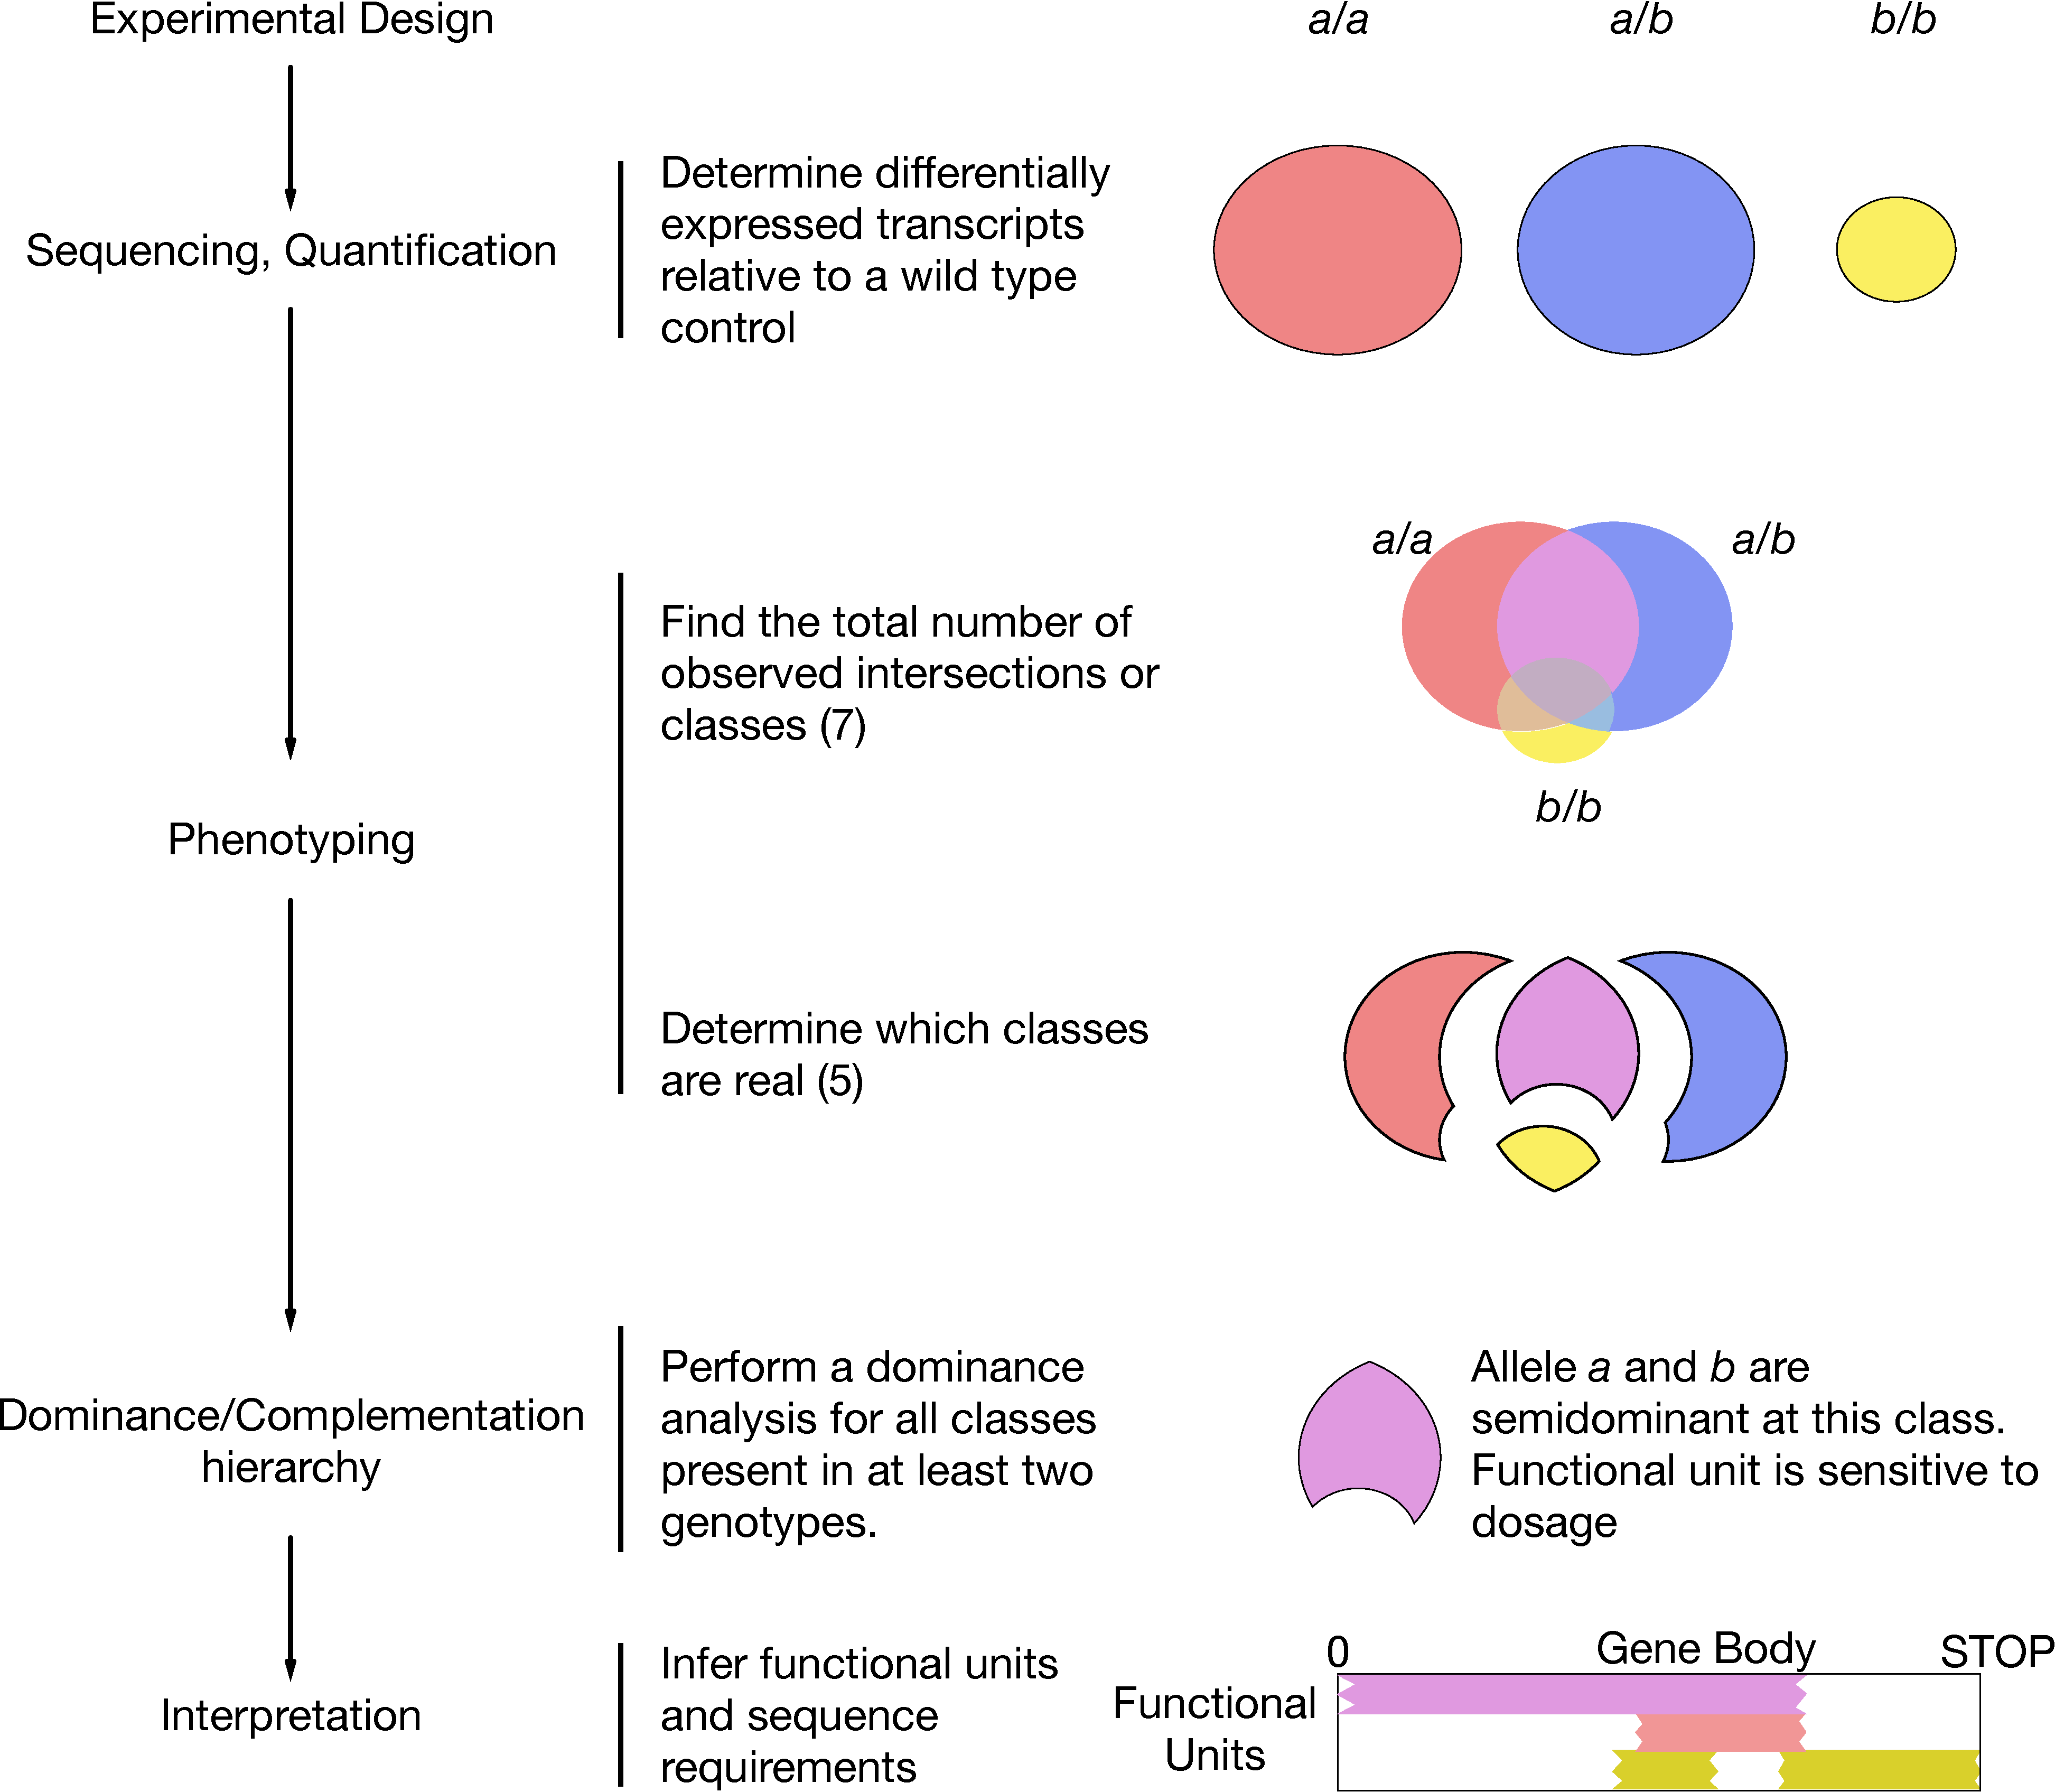
\includegraphics[width=\textwidth]{../../figs/flowchart.pdf}
  \caption{Flowchart for an analysis of arbitrary allelic series. A set of
  alleles is selected, and the corresponding genotypes are sequenced.
  Independent phenotypic classes are then identified. For each phenotypic class,
  the alleles are ordered in a dominance/complementation hierarchy, which can
  then be used to infer functional units within the genes in question.}
\label{fig:flowchart}
\end{figure*}


As a proof of principle, we sequenced in triplicate cDNA synthesized from mRNA
extracted from \emph{sy622} homozygotes, \emph{bx93} homozygotes,
\emph{trans}-heterozygotes of both alleles and wild-type controls at a depth of
20 million reads per replicate. We calculated differential expression with
respect to a wild-type control using a general linear model
(see~\nameref{sec:methods}). Differential expression with respect to the
wild-type control for each transcript $i$ in a genotype $g$ is measured via a
coefficient $\beta_{g, i}$, which can be loosely interpreted as the natural
logarithm of the fold-change. Transcripts were considered to have differential
expression between wild-type and a mutant if $q\leq 0.1$.

Using these definitions, we found \weakn{} differentially expressed genes in the
\emph{bx93} homozygote transcriptome, and \strongn{} differentially expressed
genes in the \emph{sy622} homozygote transcriptome (
see
% Fig.~\ref{fig:false_hit}; see also the
\href{https://wormlabcaltech.github.io/med-cafe/notebook/basic.html}{Basic
Statistics Notebook}). We also sequenced \emph{trans}-heterozygotic animals with
genotype \gene{dpy-6(e14) bx93/+ sy622}. The \emph{trans}-heterozygote
transcriptome had \transn{} differentially expressed genes.

% \subsection*{False hit analysis identifies four phenotypic classes}

We used a false hit analysis to identify four non-overlapping phenotypic classes.
% (see Fig.~\ref{fig:venn})
We use the term allele- or genotype-specific to refer
to groups of transcripts that are solely perturbed in a single genotype. On the
other hand, we use the term allele-associated to refer to those groups of
transcripts that are perturbed in at least two genotypes. We identified a
\textbf{\emph{sy622}-associated} phenotypic class, which consisted of 720 genes
differentially expressed in \emph{sy622} homozygotes and in
\emph{trans}-heterozygotes, but which were not differentially expressed in
\emph{bx93} homozygotes. We also identified a \textbf{\emph{bx93}-associated}
phenotypic class, which contains 403 genes. We also identified a
\textbf{\emph{sy622}-specific} phenotypic class (1,841 genes) and a
\textbf{\emph{trans}-heterozygote-specific} phenotypic class (1,226 genes; see
the
\href{https://wormlabcaltech.github.io/med-cafe/notebook/phenotypic_classes.html}{
Phenotypic Classes Notebook}).


% \begin{figure}
%   \centering{}
%   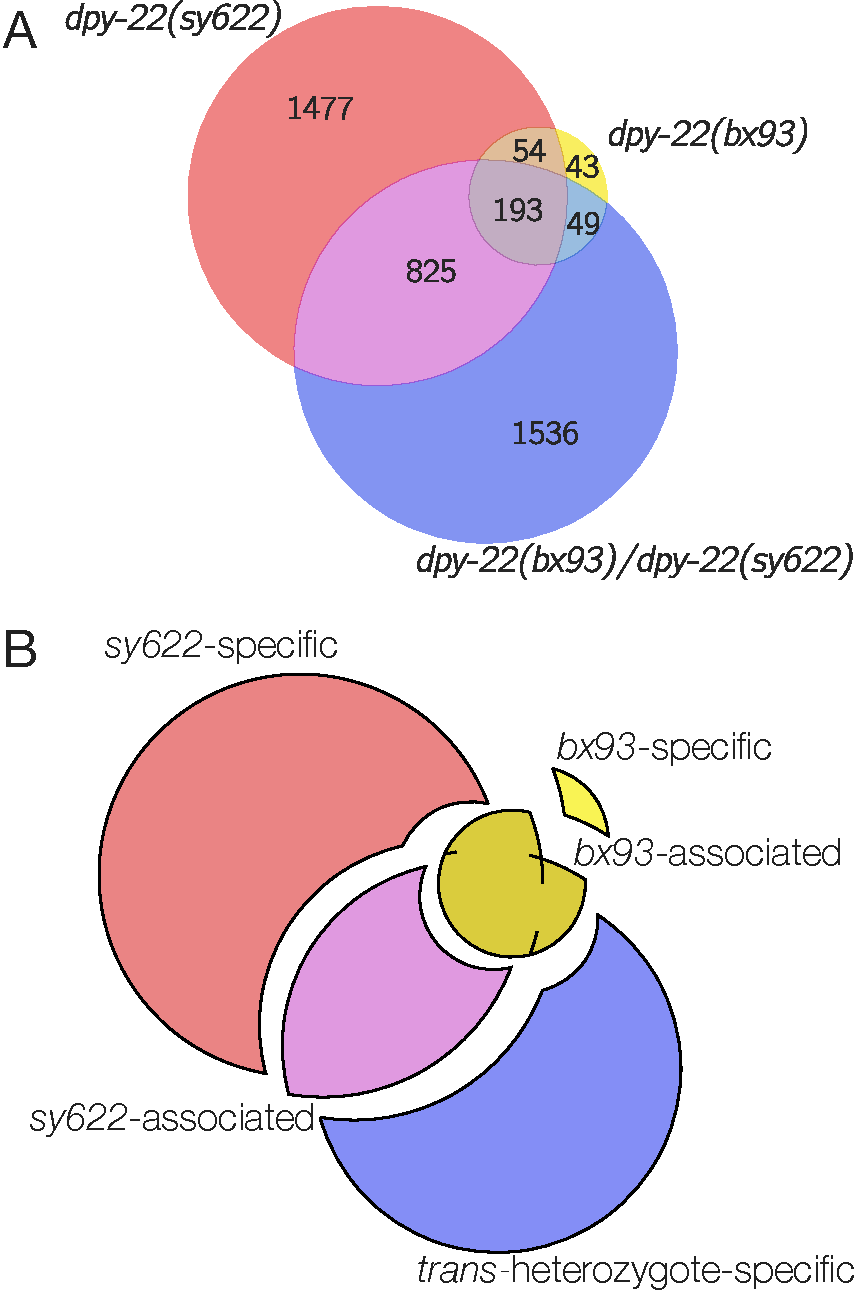
\includegraphics[width=0.45\textwidth]{../../figs/venn_diagrams.pdf}
%   \caption{
%   Transcripts under the control of \dpy{} belong to distinct phenotypic
%   classes.
%   \textbf{A} Venn diagram of genes differentially expressed in each sequenced
%   genotype relative to wild type before false hit analysis.
%   \textbf{B} Exploded Venn diagram highlighting the four identified phenotypic
%   classes after a false hit analysis.
%   }
% \label{fig:venn}
% \end{figure}


% \subsection*{Measurement of a dominance hierarchy}
To dissect these alleles, establishment of a dominance hierarchy is required for
each allele at each phenotypic class. The \emph{sy622}-specific class is
perturbed only in the \emph{sy622} homozygotes, the \emph{sy622} allele is
recessive to the \emph{bx93} allele, which has wild-type functionality for this
phenotypic class. The \emph{sy622} and \emph{bx93} alleles are semidominant
($d_{bx93} = 0.51$) to each other within this phenotypic class.  The \emph{bx93}
allele is largely but not completely dominant over the \emph{sy622} allele
($d_{bx93}=0.81$; see Table~\ref{tab:dom}).

\begin{table}
  \begin{tabular}{lc}
    \toprule
    Phenotypic Class & Dominance\\
    \midrule
    \emph{sy622}-specific & $1.00\pm0.00$\\
    \emph{sy622}-associated & $0.51\pm0.01$\\
    \emph{bx93}-associated & $0.81\pm0.01$\\
    \bottomrule
    % \midrule{}
  \end{tabular}
  \caption{Dominance analysis for the \dpy{} allelic series. Dominance values
  closer to 1 indicate \emph{bx93} is dominant over \emph{sy622}, whereas 0
  indicates \emph{sy622} is dominant over \emph{bx93}.}
\label{tab:dom}

\end{table}

% \begin{figure}
%   \centering{}
%   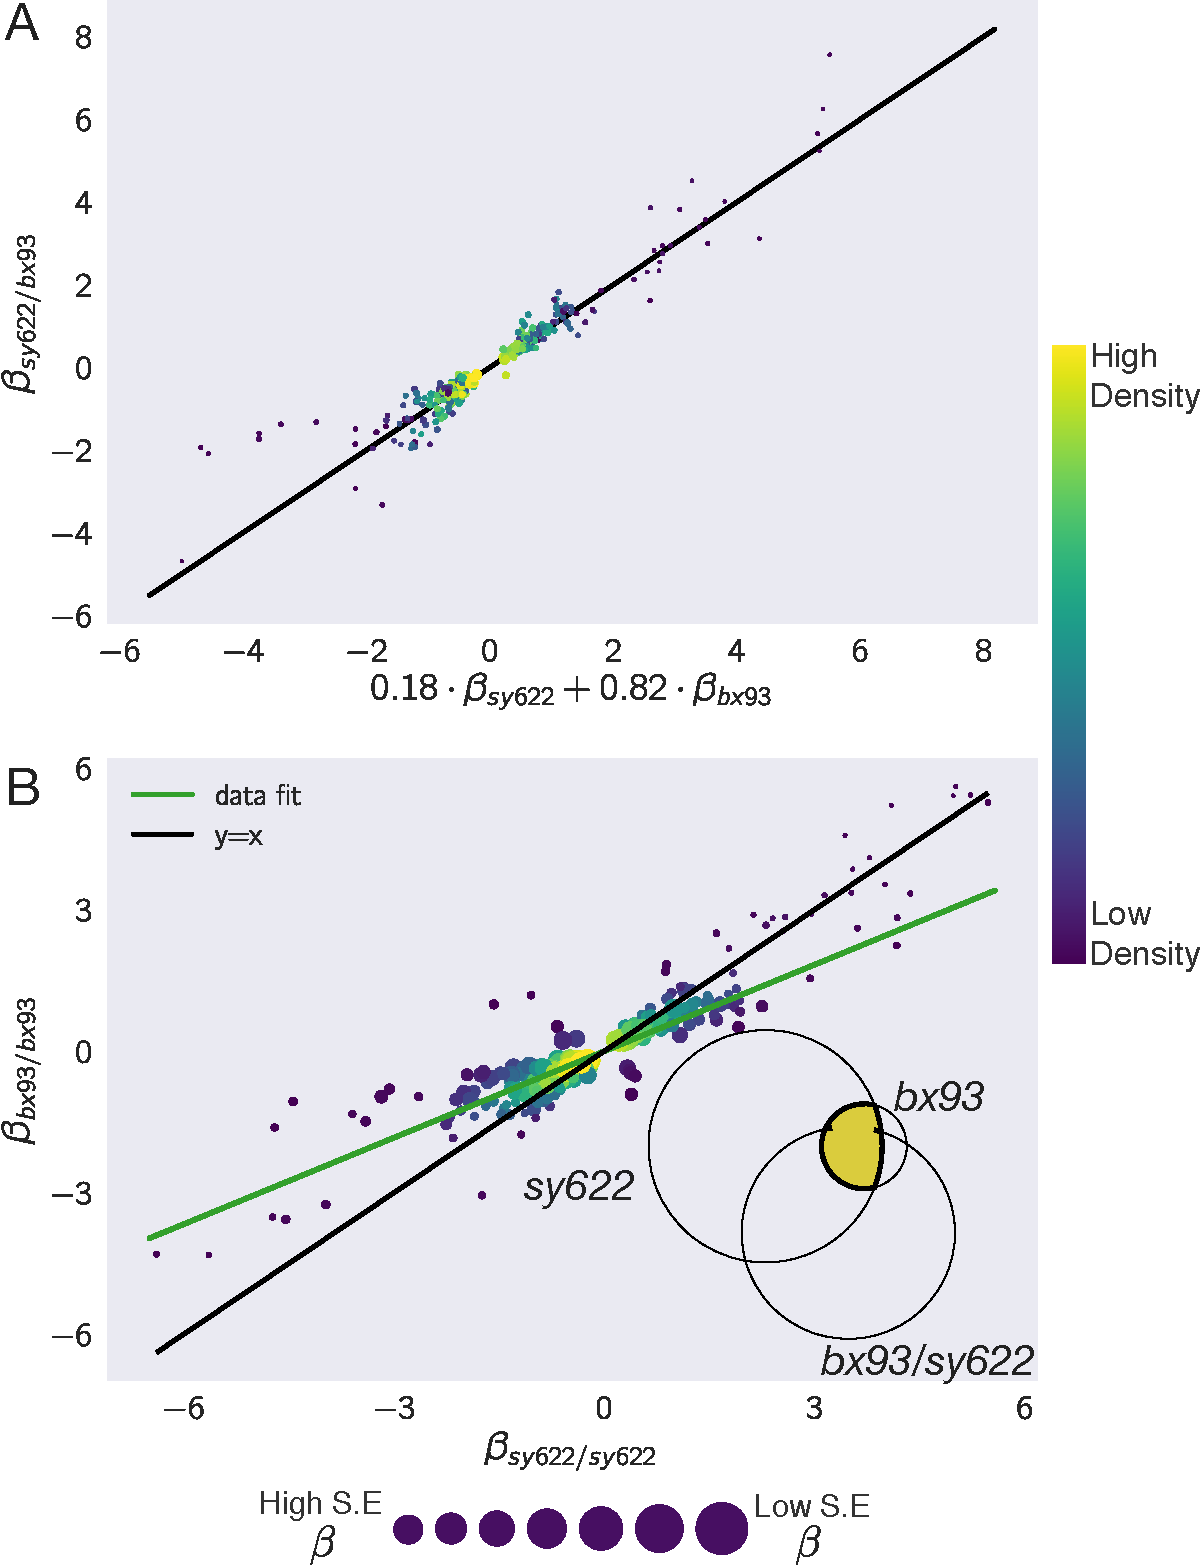
\includegraphics[width=0.5\textwidth]{../../figs/bx93_associated_analysis.pdf}
%   \caption{The \emph{bx93}-associated class has properties of both quantitative
%     and qualitative allelic series.
%     \textbf{A} In \emph{bx93}
%     homozygotes, transcripts within the \emph{bx93}-associated class are
%     less perturbed than in \emph{sy622}
%     homozygotes. The line of best fit (green) is
%     $\beta_{bx93/bx93}=0.56\cdot\beta_{sy622/sy622}$.
%     \textbf{B} In a \emph{trans}-heterozygote, the \emph{bx93} allele is largely
%     dominant over the \emph{sy622} allele for the expression levels of
%     transcripts in the \emph{bx93}-associated class.
%     In the graphs above, densely packed points are colored yellow as a visual
%     aid. The size of the point is inversely proportional to the standard error
%     of the $\beta$ coefficients.
%     }
% \label{fig:bx93_associated}
% \end{figure}



\section*{Discussion}
\label{sec:conclusions}
Our results suggest the existence of various functional units in \dpy{}
that control distinct phenotypic classes (see Fig.~\ref{fig:domains}). It seems
likely that the \emph{sy622}-specific phenotypic class is controlled by a single
functional unit, functional unit 1 (FC1), whereas the \emph{sy622}-associated
phenotypic class is controlled by a second functional unit, functional unit 2
(FC2). Although possible, it is unlikely that these functional units are
the same because the dominance behaviors are different among the two phenotypic
classes.

Although dominance analysis suggested that the \emph{bx93} allele was largely
dominant over the \emph{sy622} allele for expression levels of genes in this
class, the expression of these genes deviated from wild-type levels in both
alleles. One interpretation is that the \emph{bx93}-associated function we
observed is the joint activity of two distinct effectors, functional units 3 and
4 (FC3, FC4, see Fig.~\ref{fig:domains}). A rigorous examination of this model
requires studying alleles that mutate the region between Q1689 and Q2549 using
homozygotes and \emph{trans}-heterozygotes. Future work should be able to
establish how many functional units exist in total, and how they may interact to
drive gene expression.

\begin{figure}
  \centering{}
  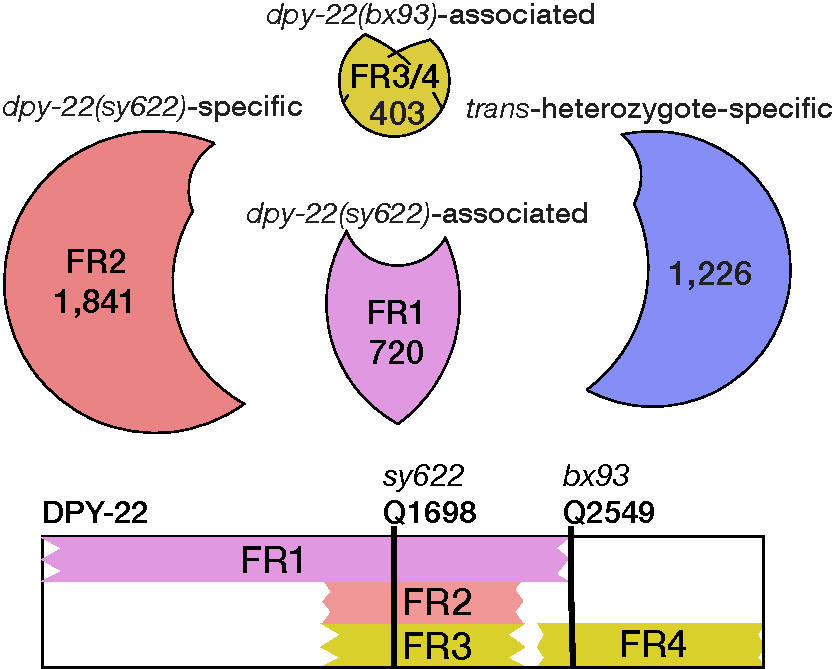
\includegraphics[width=0.5\textwidth]{../../figs/inferred_domains.pdf}
  \caption{
    The functional units associated with each phenotypic class can be
    mapped to intragenic locations. The beginning and end positions of
    these functional units are unknown,
    so edges are drawn as ragged lines. Thick horizontal lines show the
    limit where each function could end, if known. We postulate that the
    \emph{bx93}-associated class is controlled by two functional units, FC3 and
    FC4, in the tail region of this gene. Some of the units shown may be
    redundant.
  }
\label{fig:domains}
\end{figure}

In our study, we found a class of transcripts that were exclusively
differentially expressed in \emph{trans}-heterozygotes. The size of this class,
1226 genes, means it is not statistical artifact. As a result, this class
must be interpreted either as a legitimate aspect of \dpy{} biology, possibly
reflecting dosage- or tissue-specific effects, or strain-specific artifacts.
If the \emph{trans}-heterozygote specific class is not artifactual, its
biological interpretation is still unclear.
Phenotypes unique to \emph{trans}-heterozygotes are often the result of physical
interactions such as homodimerization, or dosage reduction of a toxic
product~\cite{Yook2005}. In the case of \dpy{} orthologs, how either mechanism
could operate is not obvious, since the \protein{mdt-12} is expected to assemble
in a monomeric manner into the CKM.\@ Single-cell sequencing of \cel{} has
recently been reported~\cite{Cao2017}. As this technique becomes more widely
adopted, and with decreasing cost, single-cell profiling of these genotypes may
provide information that complements the whole-organism expression phenotypes,
perhaps explaining the origin of this phenotype.

Transcriptomic phenotypes generate large amounts of information that can be used
to determine functional units. However, false positive and false negative events
occur frequently enough to create artifactual populations of transcripts.
Moreover, the distribution of false positive and false negative hits may not be
uniform across phenotypic classes or their equivalent in other experimental
designs. Identifying what classes are most at risk of these events and to what
extent these classes may be polluted by false signals will prevent
over-interpretation and may significantly decrease the apparent complexity of a
gene or a genetic interaction, because artifactual classes can often exhibit
fantastical biological behaviors (such as contrived examples of intragenic
complementation or dosage models). As a general rule, small clusters or classes
should be viewed with skepticism, particularly if the biological interpretation
is implausible. These conclusions are of broad significance to chromatin
research where highly multiplexed measurements are compared to identify
similarities and differences in the genome-wide behavior of a single variable
under multiple conditions.

We have shown that transcriptomes can be used to study allelic series to
partition the transcriptomic effects of a large, pleiotropic gene into separable
phenotypic classes that would otherwise be difficult to identify using other
methods. Given the importance of allelic series for fully characterizing
genetic pathways, we are optimistic that this method will be a useful addition
towards making full use of the potential of these molecular phenotypes.


\section*{Methods}
\label{sec:methods}
Methods, including statements of data availability and any associated
accession codes and references, are available in the online version of
the paper.

% \subsection*{Strains used}
% Strains used were N2 wild-type (Bristol),
% PS4087 \gene{mdt-12(sy622)},
% PS4187 \gene{mdt-12(bx93)},
% %line break inserted below because \gene{...} doesn't linebreak well
% and PS4176\\ \gene{dpy-6(e14) mdt-12(bx93)/ + mdt-12(sy622)}.
% Lines were grown on standard nematode growth media (NGM) Petri plates seeded
% with OP50 \ecol{} at 20\degree{}C~\cite{Brenner1974}.
%
% \subsection*{Strain synchronization, harvesting and RNA sequencing}
% Strains were synchronized by bleaching P$_0$'s into virgin S. basal (no
% cholesterol or ethanol added) for 8--12 hours. Arrested L1 larvae were placed in
% NGM plates seeded with OP50 at 20\degree{}C and grown to the young adult stage
% (assessed by vulval morphology and lack of embryos). RNA extraction was
% performed as described in~\cite{AngelesAlboresHIF} and sequenced using a
% previously described protocol~\cite{Angeles-Albores2017}.
%
% \subsection*{Read pseudo-alignment and differential expression}
% Reads were pseudo-aligned to the \cel{} genome (WBcel235) using
% Kallisto~\cite{Bray2016}, using 200 bootstraps and with the sequence bias
% (\texttt{--seqBias}) flag. The fragment size for all libraries was set to 200
% and the standard deviation to 40. Quality control was performed on a subset of
% the reads using FastQC, RNAseQC, BowTie and
% MultiQC~\cite{Andrews2010,Deluca2012,Langmead2009,Ewels2016}. All libraries had
% good quality scores.
%
% Differential expression analysis was performed using
% Sleuth~\cite{Pimentel2016a}. We used a general linear model to identify
% genes that were differentially expressed between wild-type and mutant libraries.
% To increase our statistical power, we pooled young adult wild-type replicates
% from other published~\cite{AngelesAlboresHIF,Angeles-Albores2017} and unpublished
% analysis adjusting for batch effects.
% % All wild-type replicates were collected at the same stage (young
% % adult). In total, we had 10 wild-type replicates from 4 different batches, which
% % heightened our statistical power. Batch effects were smaller than
% % between-genotype effects, as assessed by principal component analysis (PCA),
% % except when switching between samples constructed by different library methods.
% % Wild-type samples constructed using the same library method clustered together
% % and away from all other mutant samples. However, clustering wild-type samples by
% % themselves revealed that the samples clusters correlated with the person who
% % collected them. Therefore, we added batch correction terms to our model to
% % account for batch effects from library construction as well as from the person
% % who collected the samples.
%
% \subsection*{Non-parametric bootstrap}
% We performed non-parametric bootstrap testing to identify whether two
% distributions had the same test statistic using $10^6$ bootstraps.
% % Briefly, the two datasets were mixed,
% % and samples were selected at random with replacement from the mixed population
% % into two new datasets. We calculated the difference in the means of these new
% % datasets. We iterated this process $10^6$ times. To calculate a $p$-value that
% % the null hypothesis is true, we identified the number of times a difference in
% % the means of the simulated populations was greater than or equal to the observed
% % difference in the means of the real population. We divided this result by $10^6$
% % to complete the calculation for a $p$-value.
% If no statistics equal to or greater than the observed statistic was observed,
% we reported the $p$-value as $p<10^{-6}$. Otherwise, we reported
% the exact $p$-value. We chose to reject the null hypothesis that the means of
% the two datasets are equal to each other if $p < 0.05$.
%
% \subsection*{Dominance analysis}
% \label{subsec:dominance}
% We modeled allelic dominance as a weighted average of allelic activity:
% % our model proposed that $\beta$ coefficients of the heterozygote,
% % $\beta_{a/b,i,\text{Pred}}$, could be modeled as a linear combination of the
% % coefficients of each homozygote:
% \begin{equation}
%   \beta_{a/b,i,\text{Pred}}(d_a) = d_a\cdot \beta_{a/a,i} +
%                                    (1-d_a)\cdot \beta_{b/b,i},
% \end{equation}
% where $\beta_{k/k, i}$ refers to the $\beta$ value of the $i$th isoform in a
% genotype $k/k$, and $d_a$ is the dominance coefficient for allele $a$.
%
% To find the parameters $d_a$ that maximized the probability of observing the
% data, we found the parameter, $d_a$, that maximized the equation:
% \begin{equation}
%     P(d_a|D,H,I) \propto \prod_{i \in S}
%                    \exp{-\frac{{(\beta_{a/b,i,\text{Obs}} -
%                                 \beta_{a/b,i,\text{Pred}}(d_a))}^2}{
%                                 2\sigma_i^2}}
% \end{equation}
% where $\beta_{a/b,i,\text{Obs}}$ was the coefficient associated with the $i$th
% isoform in the \emph{trans}-het $a/b$ and $\sigma_i$ was the standard error of
% the $i$th isoform in the \emph{trans}-heterozygote samples as output by
% Kallisto. $S$ is the set of isoforms that participate in the regression (see
% main text). This equation describes a linear regression which was solved
% numerically.
%
% \subsection*{Code}
% Code was written in Jupyter notebooks~\cite{Perez2007} using the Python
% programming language. The Numpy, pandas and scipy libraries were used for
% computation~\cite{VanDerWalt2011,McKinney2011,Oliphant2007} and the matplotlib
% and seaborn libraries were used for data visualization~\cite{Hunter2007,Waskom}.
% Enrichment analyses were performed using the WormBase Enrichment
% Suite~\cite{Angeles-Albores2016}. For all enrichment analyses, a $q$-value of
% less than $10^{-3}$ was considered statistically significant. For gene ontology
% enrichment analysis, terms were considered statistically significant only if
% they also showed an enrichment fold-change greater than 2.
%
% \subsection*{Data Availability}
% Raw and processed reads were deposited in the Gene Expression Omnibus. Scripts
% for the entire analysis can be found with version control in our Github
% repository, \url{https://github.com/WormLabCaltech/med-cafe}. A user-friendly,
% commented website containing the complete analyses can be found at
% \url{https://wormlabcaltech.github.io/med-cafe/}. Raw reads and quantified
% abundances for each sample were deposited at the NCBI Gene Expression Omnibus
% (GEO)~\cite{Edgar2002} under the accession code GSE107523
% (\url{https://www.ncbi.nlm.nih.gov/geo/query/acc.cgi?acc=GSE107523}).

\section*{Acknowledgements}
This work was supported by HHMI with whom PWS was an investigator, by the
Millard and Muriel Jacobs Genetics and Genomics Laboratory at California
Institute of Technology, and by the NIH grant U41 HG002223. This article
would not be possible without help from Dr.\ Igor Antoshechkin and Dr.\ Vijaya
Kumar who performed the library preparation and sequencing.
% We would like to
% thank Carmie Puckett Robinson for the unpublished Dpy transcriptional
% signature.
Han Wang, Hillel Schwartz, Erich Schwarz, Porfirio Quintero and
Carmie Puckett Robinson provided valuable input throughout the project.

%This is where your bibliography is generated.
\bibliography{citations}
\bibliographystyle{naturemag}

\end{document}
